\documentclass{whiteboard}
\begin{document}
\begin{frame}[plain,t]
 \bbcover{Grafos}{Grafos Bipartidos}{Prof. Edson Alves}{Faculdade UnB Gama}
\end{frame}

\begin{frame}[plain,t]
\begin{tikzpicture}
\node[draw,opacity=0] at (0, 0) {x};
\node[draw,opacity=0] at (14, 8) {x};
 \node[anchor=west] at (0, 6) { \Large \bbbold{Grafos bipartidos} };
\end{tikzpicture}
\end{frame}

\begin{frame}[plain,t]
\begin{tikzpicture}
\node[draw,opacity=0] at (0, 0) {x};
\node[draw,opacity=0] at (14, 8) {x};
 \node[anchor=west] at (0, 6) { \Large \bbbold{Grafos bipartidos} };
 \node[anchor=west] at (1, 5) { \bbtext{Um grafo é \bbbold{bipartido} se todos os seus vértices podem ser coloridos usando} };
 \node[anchor=west] at (0.5, 4) { \bbtext{apenas duas cores, de modo que todos os pares de vértices vizinhos tenham} };
 \node[anchor=west] at (0.5, 3) { \bbtext{cores distintas.} };
\end{tikzpicture}
\end{frame}

\begin{frame}[plain,t]
\begin{tikzpicture}
\node[draw,opacity=0] at (0, 0) {x};
\node[draw,opacity=0] at (14, 8) {x};
 \node[anchor=west] at (0, 7) { \Large \bbbold{Identificação de grafos bipartidos} };
\end{tikzpicture}
\end{frame}

\begin{frame}[plain,t]
\begin{tikzpicture}
\node[draw,opacity=0] at (0, 0) {x};
\node[draw,opacity=0] at (14, 8) {x};
 \node[anchor=west] at (0, 7) { \Large \bbbold{Identificação de grafos bipartidos} };
 \node[anchor=west] at (1, 6) { $\star$ \bbtext{Um grafo bipartido pode ser identificado por meio de uma travessia} };
\end{tikzpicture}
\end{frame}

\begin{frame}[plain,t]
\begin{tikzpicture}
\node[draw,opacity=0] at (0, 0) {x};
\node[draw,opacity=0] at (14, 8) {x};
 \node[anchor=west] at (0, 7) { \Large \bbbold{Identificação de grafos bipartidos} };
 \node[anchor=west] at (1, 6) { $\star$ \bbtext{Um grafo bipartido pode ser identificado por meio de uma travessia} };
 \node[anchor=west] at (1, 5) { $\star$ \bbtext{Inicialmente não há atribuição de cores aos vértices} };
\end{tikzpicture}
\end{frame}

\begin{frame}[plain,t]
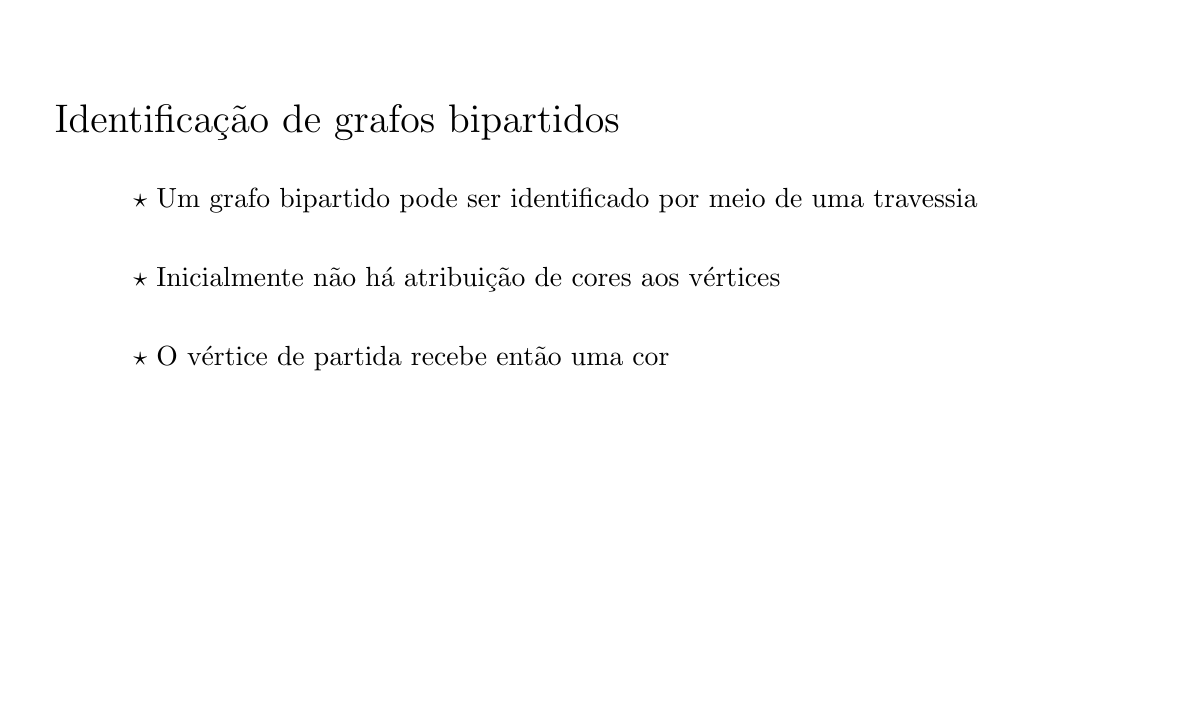
\begin{tikzpicture}
\node[draw,opacity=0] at (0, 0) {x};
\node[draw,opacity=0] at (14, 8) {x};
 \node[anchor=west] at (0, 7) { \Large \bbbold{Identificação de grafos bipartidos} };
 \node[anchor=west] at (1, 6) { $\star$ \bbtext{Um grafo bipartido pode ser identificado por meio de uma travessia} };
 \node[anchor=west] at (1, 5) { $\star$ \bbtext{Inicialmente não há atribuição de cores aos vértices} };
 \node[anchor=west] at (1, 4) { $\star$ \bbtext{O vértice de partida recebe então uma cor} };
\end{tikzpicture}
\end{frame}

\begin{frame}[plain,t]
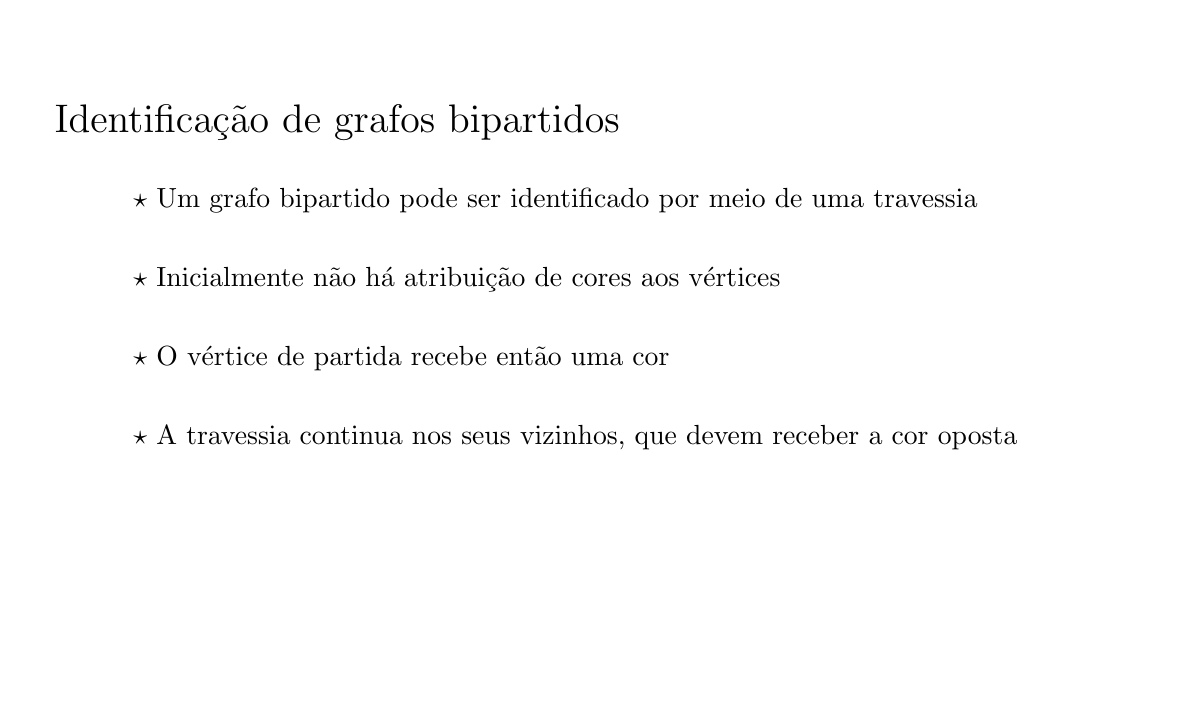
\begin{tikzpicture}
\node[draw,opacity=0] at (0, 0) {x};
\node[draw,opacity=0] at (14, 8) {x};
 \node[anchor=west] at (0, 7) { \Large \bbbold{Identificação de grafos bipartidos} };
 \node[anchor=west] at (1, 6) { $\star$ \bbtext{Um grafo bipartido pode ser identificado por meio de uma travessia} };
 \node[anchor=west] at (1, 5) { $\star$ \bbtext{Inicialmente não há atribuição de cores aos vértices} };
 \node[anchor=west] at (1, 4) { $\star$ \bbtext{O vértice de partida recebe então uma cor} };
 \node[anchor=west] at (1, 3) { $\star$ \bbtext{A travessia continua nos seus vizinhos, que devem receber a cor oposta} };
\end{tikzpicture}
\end{frame}

\begin{frame}[plain,t]
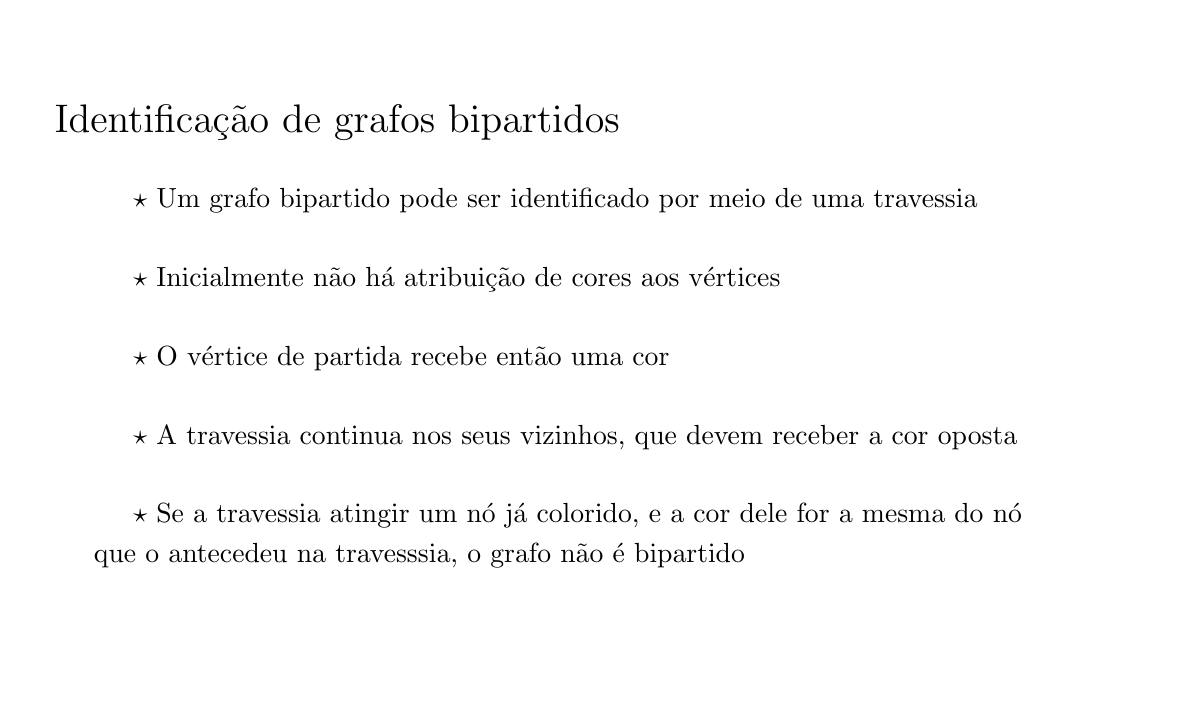
\begin{tikzpicture}
\node[draw,opacity=0] at (0, 0) {x};
\node[draw,opacity=0] at (14, 8) {x};
 \node[anchor=west] at (0, 7) { \Large \bbbold{Identificação de grafos bipartidos} };
 \node[anchor=west] at (1, 6) { $\star$ \bbtext{Um grafo bipartido pode ser identificado por meio de uma travessia} };
 \node[anchor=west] at (1, 5) { $\star$ \bbtext{Inicialmente não há atribuição de cores aos vértices} };
 \node[anchor=west] at (1, 4) { $\star$ \bbtext{O vértice de partida recebe então uma cor} };
 \node[anchor=west] at (1, 3) { $\star$ \bbtext{A travessia continua nos seus vizinhos, que devem receber a cor oposta} };
 \node[anchor=west] at (1, 2) { $\star$ \bbtext{Se a travessia atingir um nó já colorido, e a cor dele for a mesma do nó} };
 \node[anchor=west] at (0.5, 1.5) { \bbtext{que o antecedeu na travesssia, o grafo não é bipartido} };
\end{tikzpicture}
\end{frame}

\begin{frame}[plain,t]
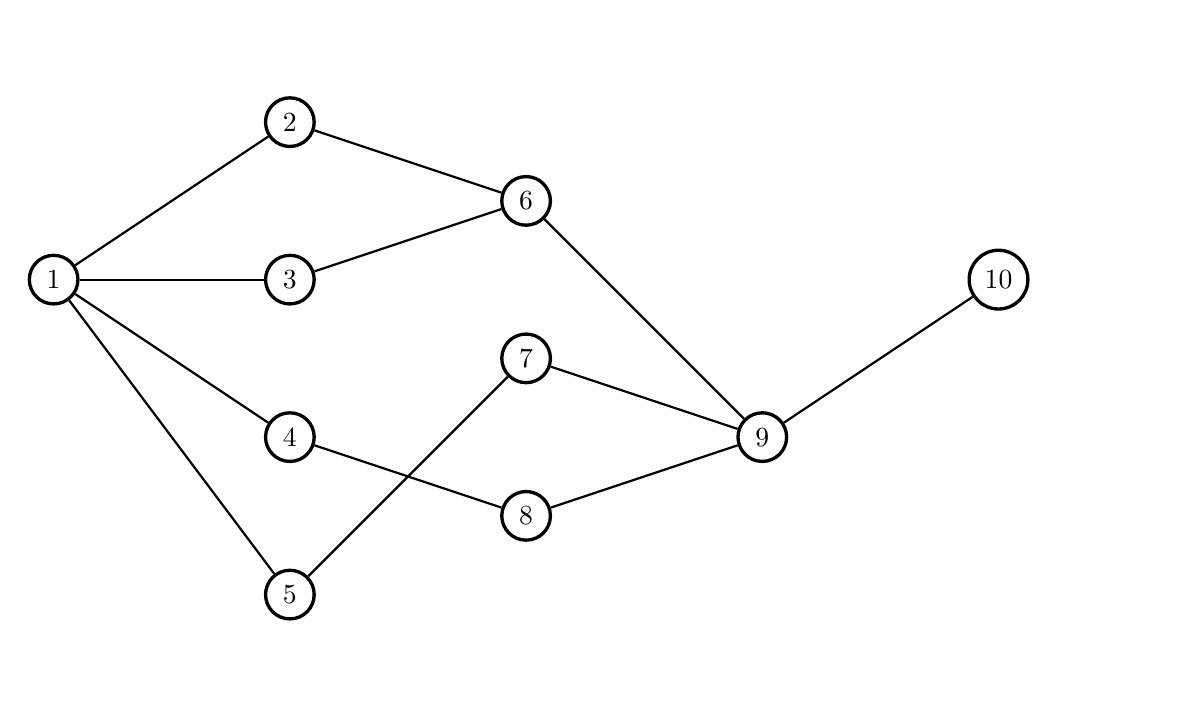
\begin{tikzpicture}
\node[draw,opacity=0] at (0, 0) {x};
\node[draw,opacity=0] at (14, 8) {x};
 \node[circle, draw, very thick] (A) at (0, 5) { \bbtext{1} };
 \node[circle, draw, very thick] (B) at (3, 7) { \bbtext{2} };
 \node[circle, draw, very thick] (C) at (3, 5) { \bbtext{3} };
 \node[circle, draw, very thick] (D) at (3, 3) { \bbtext{4} };
 \node[circle, draw, very thick] (E) at (3, 1) { \bbtext{5} };
 \node[circle, draw, very thick] (F) at (6, 6) { \bbtext{6} };
 \node[circle, draw, very thick] (G) at (6, 4) { \bbtext{7} };
 \node[circle, draw, very thick] (H) at (6, 2) { \bbtext{8} };
 \node[circle, draw, very thick] (I) at (9, 3) { \bbtext{9} };
 \node[circle, draw, very thick] (J) at (12, 5) { \bbtext{10} };
 \draw[thick] (A) to (B);
 \draw[thick] (A) to (C);
 \draw[thick] (A) to (D);
 \draw[thick] (A) to (E);
 \draw[thick] (B) to (F);
 \draw[thick] (C) to (F);
 \draw[thick] (D) to (H);
 \draw[thick] (E) to (G);
 \draw[thick] (F) to (I);
 \draw[thick] (G) to (I);
 \draw[thick] (H) to (I);
 \draw[thick] (I) to (J);
\end{tikzpicture}
\end{frame}

\begin{frame}[plain,t]
\begin{tikzpicture}
\node[draw,opacity=0] at (0, 0) {x};
\node[draw,opacity=0] at (14, 8) {x};
 \node[circle, draw, very thick] (B) at (3, 7) { \bbtext{2} };
 \node[circle, draw, very thick] (C) at (3, 5) { \bbtext{3} };
 \node[circle, draw, very thick] (D) at (3, 3) { \bbtext{4} };
 \node[circle, draw, very thick] (E) at (3, 1) { \bbtext{5} };
 \node[circle, draw, very thick] (F) at (6, 6) { \bbtext{6} };
 \node[circle, draw, very thick] (G) at (6, 4) { \bbtext{7} };
 \node[circle, draw, very thick] (H) at (6, 2) { \bbtext{8} };
 \node[circle, draw, very thick] (I) at (9, 3) { \bbtext{9} };
 \node[circle, draw, very thick] (J) at (12, 5) { \bbtext{10} };
 \draw[thick] (A) to (B);
 \draw[thick] (A) to (C);
 \draw[thick] (A) to (D);
 \draw[thick] (A) to (E);
 \draw[thick] (B) to (F);
 \draw[thick] (C) to (F);
 \draw[thick] (D) to (H);
 \draw[thick] (E) to (G);
 \draw[thick] (F) to (I);
 \draw[thick] (G) to (I);
 \draw[thick] (H) to (I);
 \draw[thick] (I) to (J);
 \node[circle, fill, color=BBCyan] (A) at (0, 5) { \bbtext{1} };
 \node[circle, draw, very thick] (A) at (0, 5) { \bbtext{1} };
\end{tikzpicture}
\end{frame}

\begin{frame}[plain,t]
\begin{tikzpicture}
\node[draw,opacity=0] at (0, 0) {x};
\node[draw,opacity=0] at (14, 8) {x};
 \node[circle, draw, very thick] (C) at (3, 5) { \bbtext{3} };
 \node[circle, draw, very thick] (D) at (3, 3) { \bbtext{4} };
 \node[circle, draw, very thick] (E) at (3, 1) { \bbtext{5} };
 \node[circle, draw, very thick] (F) at (6, 6) { \bbtext{6} };
 \node[circle, draw, very thick] (G) at (6, 4) { \bbtext{7} };
 \node[circle, draw, very thick] (H) at (6, 2) { \bbtext{8} };
 \node[circle, draw, very thick] (I) at (9, 3) { \bbtext{9} };
 \node[circle, draw, very thick] (J) at (12, 5) { \bbtext{10} };
 \draw[thick] (A) to (C);
 \draw[thick] (A) to (D);
 \draw[thick] (A) to (E);
 \draw[thick] (B) to (F);
 \draw[thick] (C) to (F);
 \draw[thick] (D) to (H);
 \draw[thick] (E) to (G);
 \draw[thick] (F) to (I);
 \draw[thick] (G) to (I);
 \draw[thick] (H) to (I);
 \draw[thick] (I) to (J);
 \node[circle, fill, color=BBCyan] (A) at (0, 5) { \bbtext{1} };
 \node[circle, draw, very thick] (A) at (0, 5) { \bbtext{1} };
 \node[circle, fill, color=BBOrange] (B) at (3, 7) { \bbtext{2} };
 \node[circle, draw, very thick] (B) at (3, 7) { \bbtext{2} };
 \draw[-latex,very thick] (A) to (B);
\end{tikzpicture}
\end{frame}

\begin{frame}[plain,t]
\begin{tikzpicture}
\node[draw,opacity=0] at (0, 0) {x};
\node[draw,opacity=0] at (14, 8) {x};
 \node[circle, draw, very thick] (C) at (3, 5) { \bbtext{3} };
 \node[circle, draw, very thick] (D) at (3, 3) { \bbtext{4} };
 \node[circle, draw, very thick] (E) at (3, 1) { \bbtext{5} };
 \node[circle, draw, very thick] (G) at (6, 4) { \bbtext{7} };
 \node[circle, draw, very thick] (H) at (6, 2) { \bbtext{8} };
 \node[circle, draw, very thick] (I) at (9, 3) { \bbtext{9} };
 \node[circle, draw, very thick] (J) at (12, 5) { \bbtext{10} };
 \draw[thick] (A) to (C);
 \draw[thick] (A) to (D);
 \draw[thick] (A) to (E);
 \draw[thick] (C) to (F);
 \draw[thick] (D) to (H);
 \draw[thick] (E) to (G);
 \draw[thick] (F) to (I);
 \draw[thick] (G) to (I);
 \draw[thick] (H) to (I);
 \draw[thick] (I) to (J);
 \node[circle, fill, color=BBCyan] (A) at (0, 5) { \bbtext{1} };
 \node[circle, draw, very thick] (A) at (0, 5) { \bbtext{1} };
 \node[circle, fill, color=BBOrange] (B) at (3, 7) { \bbtext{2} };
 \node[circle, draw, very thick] (B) at (3, 7) { \bbtext{2} };
 \draw[-latex,very thick] (A) to (B);
 \node[circle, fill, color=BBCyan] (F) at (6, 6) { \bbtext{6} };
 \node[circle, draw, very thick] (F) at (6, 6) { \bbtext{6} };
 \draw[-latex,very thick] (B) to (F);
\end{tikzpicture}
\end{frame}

\begin{frame}[plain,t]
\begin{tikzpicture}
\node[draw,opacity=0] at (0, 0) {x};
\node[draw,opacity=0] at (14, 8) {x};
 \node[circle, draw, very thick] (D) at (3, 3) { \bbtext{4} };
 \node[circle, draw, very thick] (E) at (3, 1) { \bbtext{5} };
 \node[circle, draw, very thick] (G) at (6, 4) { \bbtext{7} };
 \node[circle, draw, very thick] (H) at (6, 2) { \bbtext{8} };
 \node[circle, draw, very thick] (I) at (9, 3) { \bbtext{9} };
 \node[circle, draw, very thick] (J) at (12, 5) { \bbtext{10} };
 \draw[thick] (A) to (C);
 \draw[thick] (A) to (D);
 \draw[thick] (A) to (E);
 \draw[thick] (D) to (H);
 \draw[thick] (E) to (G);
 \draw[thick] (F) to (I);
 \draw[thick] (G) to (I);
 \draw[thick] (H) to (I);
 \draw[thick] (I) to (J);
 \node[circle, fill, color=BBCyan] (A) at (0, 5) { \bbtext{1} };
 \node[circle, draw, very thick] (A) at (0, 5) { \bbtext{1} };
 \node[circle, fill, color=BBOrange] (B) at (3, 7) { \bbtext{2} };
 \node[circle, draw, very thick] (B) at (3, 7) { \bbtext{2} };
 \draw[-latex,very thick] (A) to (B);
 \node[circle, fill, color=BBCyan] (F) at (6, 6) { \bbtext{6} };
 \node[circle, draw, very thick] (F) at (6, 6) { \bbtext{6} };
 \draw[-latex,very thick] (B) to (F);
 \node[circle, fill, color=BBOrange] (C) at (3, 5) { \bbtext{3} };
 \node[circle, draw, very thick] (C) at (3, 5) { \bbtext{3} };
 \draw[latex-,very thick] (C) to (F);
\end{tikzpicture}
\end{frame}

\begin{frame}[plain,t]
\begin{tikzpicture}
\node[draw,opacity=0] at (0, 0) {x};
\node[draw,opacity=0] at (14, 8) {x};
 \node[circle, draw, very thick] (D) at (3, 3) { \bbtext{4} };
 \node[circle, draw, very thick] (E) at (3, 1) { \bbtext{5} };
 \node[circle, draw, very thick] (G) at (6, 4) { \bbtext{7} };
 \node[circle, draw, very thick] (H) at (6, 2) { \bbtext{8} };
 \node[circle, draw, very thick] (I) at (9, 3) { \bbtext{9} };
 \node[circle, draw, very thick] (J) at (12, 5) { \bbtext{10} };
 \draw[thick] (A) to (D);
 \draw[thick] (A) to (E);
 \draw[thick] (D) to (H);
 \draw[thick] (E) to (G);
 \draw[thick] (F) to (I);
 \draw[thick] (G) to (I);
 \draw[thick] (H) to (I);
 \draw[thick] (I) to (J);
 \node[circle, fill, color=BBCyan] (A) at (0, 5) { \bbtext{1} };
 \node[circle, draw, very thick] (A) at (0, 5) { \bbtext{1} };
 \node[circle, fill, color=BBOrange] (B) at (3, 7) { \bbtext{2} };
 \node[circle, draw, very thick] (B) at (3, 7) { \bbtext{2} };
 \draw[-latex,very thick] (A) to (B);
 \node[circle, fill, color=BBCyan] (F) at (6, 6) { \bbtext{6} };
 \node[circle, draw, very thick] (F) at (6, 6) { \bbtext{6} };
 \draw[-latex,very thick] (B) to (F);
 \node[circle, fill, color=BBOrange] (C) at (3, 5) { \bbtext{3} };
 \node[circle, draw, very thick] (C) at (3, 5) { \bbtext{3} };
 \draw[latex-,very thick] (C) to (F);
 \draw[latex-,very thick,dashed] (A) to (C);
\end{tikzpicture}
\end{frame}

\begin{frame}[plain,t]
\begin{tikzpicture}
\node[draw,opacity=0] at (0, 0) {x};
\node[draw,opacity=0] at (14, 8) {x};
 \node[circle, draw, very thick] (D) at (3, 3) { \bbtext{4} };
 \node[circle, draw, very thick] (E) at (3, 1) { \bbtext{5} };
 \node[circle, draw, very thick] (G) at (6, 4) { \bbtext{7} };
 \node[circle, draw, very thick] (H) at (6, 2) { \bbtext{8} };
 \node[circle, draw, very thick] (J) at (12, 5) { \bbtext{10} };
 \draw[thick] (A) to (D);
 \draw[thick] (A) to (E);
 \draw[thick] (D) to (H);
 \draw[thick] (E) to (G);
 \draw[thick] (G) to (I);
 \draw[thick] (H) to (I);
 \draw[thick] (I) to (J);
 \node[circle, fill, color=BBCyan] (A) at (0, 5) { \bbtext{1} };
 \node[circle, draw, very thick] (A) at (0, 5) { \bbtext{1} };
 \node[circle, fill, color=BBOrange] (B) at (3, 7) { \bbtext{2} };
 \node[circle, draw, very thick] (B) at (3, 7) { \bbtext{2} };
 \draw[-latex,very thick] (A) to (B);
 \node[circle, fill, color=BBCyan] (F) at (6, 6) { \bbtext{6} };
 \node[circle, draw, very thick] (F) at (6, 6) { \bbtext{6} };
 \draw[-latex,very thick] (B) to (F);
 \node[circle, fill, color=BBOrange] (C) at (3, 5) { \bbtext{3} };
 \node[circle, draw, very thick] (C) at (3, 5) { \bbtext{3} };
 \draw[latex-,very thick] (C) to (F);
 \draw[latex-,very thick,dashed] (A) to (C);
 \node[circle, fill, color=BBOrange] (I) at (9, 3) { \bbtext{9} };
 \node[circle, draw, very thick] (I) at (9, 3) { \bbtext{9} };
 \draw[-latex,very thick] (F) to (I);
\end{tikzpicture}
\end{frame}

\begin{frame}[plain,t]
\begin{tikzpicture}
\node[draw,opacity=0] at (0, 0) {x};
\node[draw,opacity=0] at (14, 8) {x};
 \node[circle, draw, very thick] (D) at (3, 3) { \bbtext{4} };
 \node[circle, draw, very thick] (E) at (3, 1) { \bbtext{5} };
 \node[circle, draw, very thick] (H) at (6, 2) { \bbtext{8} };
 \node[circle, draw, very thick] (J) at (12, 5) { \bbtext{10} };
 \draw[thick] (A) to (D);
 \draw[thick] (A) to (E);
 \draw[thick] (D) to (H);
 \draw[thick] (E) to (G);
 \draw[thick] (H) to (I);
 \draw[thick] (I) to (J);
 \node[circle, fill, color=BBCyan] (A) at (0, 5) { \bbtext{1} };
 \node[circle, draw, very thick] (A) at (0, 5) { \bbtext{1} };
 \node[circle, fill, color=BBOrange] (B) at (3, 7) { \bbtext{2} };
 \node[circle, draw, very thick] (B) at (3, 7) { \bbtext{2} };
 \draw[-latex,very thick] (A) to (B);
 \node[circle, fill, color=BBCyan] (F) at (6, 6) { \bbtext{6} };
 \node[circle, draw, very thick] (F) at (6, 6) { \bbtext{6} };
 \draw[-latex,very thick] (B) to (F);
 \node[circle, fill, color=BBOrange] (C) at (3, 5) { \bbtext{3} };
 \node[circle, draw, very thick] (C) at (3, 5) { \bbtext{3} };
 \draw[latex-,very thick] (C) to (F);
 \draw[latex-,very thick,dashed] (A) to (C);
 \node[circle, fill, color=BBOrange] (I) at (9, 3) { \bbtext{9} };
 \node[circle, draw, very thick] (I) at (9, 3) { \bbtext{9} };
 \draw[-latex,very thick] (F) to (I);
 \node[circle, fill, color=BBCyan] (G) at (6, 4) { \bbtext{7} };
 \node[circle, draw, very thick] (G) at (6, 4) { \bbtext{7} };
 \draw[latex-,very thick] (G) to (I);
\end{tikzpicture}
\end{frame}

\begin{frame}[plain,t]
\begin{tikzpicture}
\node[draw,opacity=0] at (0, 0) {x};
\node[draw,opacity=0] at (14, 8) {x};
 \node[circle, draw, very thick] (D) at (3, 3) { \bbtext{4} };
 \node[circle, draw, very thick] (H) at (6, 2) { \bbtext{8} };
 \node[circle, draw, very thick] (J) at (12, 5) { \bbtext{10} };
 \draw[thick] (A) to (D);
 \draw[thick] (A) to (E);
 \draw[thick] (D) to (H);
 \draw[thick] (H) to (I);
 \draw[thick] (I) to (J);
 \node[circle, fill, color=BBCyan] (A) at (0, 5) { \bbtext{1} };
 \node[circle, draw, very thick] (A) at (0, 5) { \bbtext{1} };
 \node[circle, fill, color=BBOrange] (B) at (3, 7) { \bbtext{2} };
 \node[circle, draw, very thick] (B) at (3, 7) { \bbtext{2} };
 \draw[-latex,very thick] (A) to (B);
 \node[circle, fill, color=BBCyan] (F) at (6, 6) { \bbtext{6} };
 \node[circle, draw, very thick] (F) at (6, 6) { \bbtext{6} };
 \draw[-latex,very thick] (B) to (F);
 \node[circle, fill, color=BBOrange] (C) at (3, 5) { \bbtext{3} };
 \node[circle, draw, very thick] (C) at (3, 5) { \bbtext{3} };
 \draw[latex-,very thick] (C) to (F);
 \draw[latex-,very thick,dashed] (A) to (C);
 \node[circle, fill, color=BBOrange] (I) at (9, 3) { \bbtext{9} };
 \node[circle, draw, very thick] (I) at (9, 3) { \bbtext{9} };
 \draw[-latex,very thick] (F) to (I);
 \node[circle, fill, color=BBCyan] (G) at (6, 4) { \bbtext{7} };
 \node[circle, draw, very thick] (G) at (6, 4) { \bbtext{7} };
 \draw[latex-,very thick] (G) to (I);
 \node[circle, fill, color=BBOrange] (E) at (3, 1) { \bbtext{5} };
 \node[circle, draw, very thick] (E) at (3, 1) { \bbtext{5} };
 \draw[latex-,very thick] (E) to (G);
\end{tikzpicture}
\end{frame}

\begin{frame}[plain,t]
\begin{tikzpicture}
\node[draw,opacity=0] at (0, 0) {x};
\node[draw,opacity=0] at (14, 8) {x};
 \node[circle, draw, very thick] (D) at (3, 3) { \bbtext{4} };
 \node[circle, draw, very thick] (H) at (6, 2) { \bbtext{8} };
 \node[circle, draw, very thick] (J) at (12, 5) { \bbtext{10} };
 \draw[thick] (A) to (D);
 \draw[thick] (D) to (H);
 \draw[thick] (H) to (I);
 \draw[thick] (I) to (J);
 \node[circle, fill, color=BBCyan] (A) at (0, 5) { \bbtext{1} };
 \node[circle, draw, very thick] (A) at (0, 5) { \bbtext{1} };
 \node[circle, fill, color=BBOrange] (B) at (3, 7) { \bbtext{2} };
 \node[circle, draw, very thick] (B) at (3, 7) { \bbtext{2} };
 \draw[-latex,very thick] (A) to (B);
 \node[circle, fill, color=BBCyan] (F) at (6, 6) { \bbtext{6} };
 \node[circle, draw, very thick] (F) at (6, 6) { \bbtext{6} };
 \draw[-latex,very thick] (B) to (F);
 \node[circle, fill, color=BBOrange] (C) at (3, 5) { \bbtext{3} };
 \node[circle, draw, very thick] (C) at (3, 5) { \bbtext{3} };
 \draw[latex-,very thick] (C) to (F);
 \draw[latex-,very thick,dashed] (A) to (C);
 \node[circle, fill, color=BBOrange] (I) at (9, 3) { \bbtext{9} };
 \node[circle, draw, very thick] (I) at (9, 3) { \bbtext{9} };
 \draw[-latex,very thick] (F) to (I);
 \node[circle, fill, color=BBCyan] (G) at (6, 4) { \bbtext{7} };
 \node[circle, draw, very thick] (G) at (6, 4) { \bbtext{7} };
 \draw[latex-,very thick] (G) to (I);
 \node[circle, fill, color=BBOrange] (E) at (3, 1) { \bbtext{5} };
 \node[circle, draw, very thick] (E) at (3, 1) { \bbtext{5} };
 \draw[latex-,very thick] (E) to (G);
 \draw[latex-,very thick,dashed] (A) to (E);
\end{tikzpicture}
\end{frame}

\begin{frame}[plain,t]
\begin{tikzpicture}
\node[draw,opacity=0] at (0, 0) {x};
\node[draw,opacity=0] at (14, 8) {x};
 \node[circle, draw, very thick] (D) at (3, 3) { \bbtext{4} };
 \node[circle, draw, very thick] (J) at (12, 5) { \bbtext{10} };
 \draw[thick] (A) to (D);
 \draw[thick] (D) to (H);
 \draw[thick] (I) to (J);
 \node[circle, fill, color=BBCyan] (A) at (0, 5) { \bbtext{1} };
 \node[circle, draw, very thick] (A) at (0, 5) { \bbtext{1} };
 \node[circle, fill, color=BBOrange] (B) at (3, 7) { \bbtext{2} };
 \node[circle, draw, very thick] (B) at (3, 7) { \bbtext{2} };
 \draw[-latex,very thick] (A) to (B);
 \node[circle, fill, color=BBCyan] (F) at (6, 6) { \bbtext{6} };
 \node[circle, draw, very thick] (F) at (6, 6) { \bbtext{6} };
 \draw[-latex,very thick] (B) to (F);
 \node[circle, fill, color=BBOrange] (C) at (3, 5) { \bbtext{3} };
 \node[circle, draw, very thick] (C) at (3, 5) { \bbtext{3} };
 \draw[latex-,very thick] (C) to (F);
 \draw[latex-,very thick,dashed] (A) to (C);
 \node[circle, fill, color=BBOrange] (I) at (9, 3) { \bbtext{9} };
 \node[circle, draw, very thick] (I) at (9, 3) { \bbtext{9} };
 \draw[-latex,very thick] (F) to (I);
 \node[circle, fill, color=BBCyan] (G) at (6, 4) { \bbtext{7} };
 \node[circle, draw, very thick] (G) at (6, 4) { \bbtext{7} };
 \draw[latex-,very thick] (G) to (I);
 \node[circle, fill, color=BBOrange] (E) at (3, 1) { \bbtext{5} };
 \node[circle, draw, very thick] (E) at (3, 1) { \bbtext{5} };
 \draw[latex-,very thick] (E) to (G);
 \draw[latex-,very thick,dashed] (A) to (E);
 \node[circle, fill, color=BBCyan] (H) at (6, 2) { \bbtext{8} };
 \node[circle, draw, very thick] (H) at (6, 2) { \bbtext{8} };
 \draw[latex-,very thick] (H) to (I);
\end{tikzpicture}
\end{frame}

\begin{frame}[plain,t]
\begin{tikzpicture}
\node[draw,opacity=0] at (0, 0) {x};
\node[draw,opacity=0] at (14, 8) {x};
 \node[circle, draw, very thick] (J) at (12, 5) { \bbtext{10} };
 \draw[thick] (A) to (D);
 \draw[thick] (I) to (J);
 \node[circle, fill, color=BBCyan] (A) at (0, 5) { \bbtext{1} };
 \node[circle, draw, very thick] (A) at (0, 5) { \bbtext{1} };
 \node[circle, fill, color=BBOrange] (B) at (3, 7) { \bbtext{2} };
 \node[circle, draw, very thick] (B) at (3, 7) { \bbtext{2} };
 \draw[-latex,very thick] (A) to (B);
 \node[circle, fill, color=BBCyan] (F) at (6, 6) { \bbtext{6} };
 \node[circle, draw, very thick] (F) at (6, 6) { \bbtext{6} };
 \draw[-latex,very thick] (B) to (F);
 \node[circle, fill, color=BBOrange] (C) at (3, 5) { \bbtext{3} };
 \node[circle, draw, very thick] (C) at (3, 5) { \bbtext{3} };
 \draw[latex-,very thick] (C) to (F);
 \draw[latex-,very thick,dashed] (A) to (C);
 \node[circle, fill, color=BBOrange] (I) at (9, 3) { \bbtext{9} };
 \node[circle, draw, very thick] (I) at (9, 3) { \bbtext{9} };
 \draw[-latex,very thick] (F) to (I);
 \node[circle, fill, color=BBCyan] (G) at (6, 4) { \bbtext{7} };
 \node[circle, draw, very thick] (G) at (6, 4) { \bbtext{7} };
 \draw[latex-,very thick] (G) to (I);
 \node[circle, fill, color=BBOrange] (E) at (3, 1) { \bbtext{5} };
 \node[circle, draw, very thick] (E) at (3, 1) { \bbtext{5} };
 \draw[latex-,very thick] (E) to (G);
 \draw[latex-,very thick,dashed] (A) to (E);
 \node[circle, fill, color=BBCyan] (H) at (6, 2) { \bbtext{8} };
 \node[circle, draw, very thick] (H) at (6, 2) { \bbtext{8} };
 \draw[latex-,very thick] (H) to (I);
 \node[circle, fill, color=BBOrange] (D) at (3, 3) { \bbtext{4} };
 \node[circle, draw, very thick] (D) at (3, 3) { \bbtext{4} };
 \draw[latex-,very thick] (D) to (H);
\end{tikzpicture}
\end{frame}

\begin{frame}[plain,t]
\begin{tikzpicture}
\node[draw,opacity=0] at (0, 0) {x};
\node[draw,opacity=0] at (14, 8) {x};
 \node[circle, draw, very thick] (J) at (12, 5) { \bbtext{10} };
 \draw[thick] (I) to (J);
 \node[circle, fill, color=BBCyan] (A) at (0, 5) { \bbtext{1} };
 \node[circle, draw, very thick] (A) at (0, 5) { \bbtext{1} };
 \node[circle, fill, color=BBOrange] (B) at (3, 7) { \bbtext{2} };
 \node[circle, draw, very thick] (B) at (3, 7) { \bbtext{2} };
 \draw[-latex,very thick] (A) to (B);
 \node[circle, fill, color=BBCyan] (F) at (6, 6) { \bbtext{6} };
 \node[circle, draw, very thick] (F) at (6, 6) { \bbtext{6} };
 \draw[-latex,very thick] (B) to (F);
 \node[circle, fill, color=BBOrange] (C) at (3, 5) { \bbtext{3} };
 \node[circle, draw, very thick] (C) at (3, 5) { \bbtext{3} };
 \draw[latex-,very thick] (C) to (F);
 \draw[latex-,very thick,dashed] (A) to (C);
 \node[circle, fill, color=BBOrange] (I) at (9, 3) { \bbtext{9} };
 \node[circle, draw, very thick] (I) at (9, 3) { \bbtext{9} };
 \draw[-latex,very thick] (F) to (I);
 \node[circle, fill, color=BBCyan] (G) at (6, 4) { \bbtext{7} };
 \node[circle, draw, very thick] (G) at (6, 4) { \bbtext{7} };
 \draw[latex-,very thick] (G) to (I);
 \node[circle, fill, color=BBOrange] (E) at (3, 1) { \bbtext{5} };
 \node[circle, draw, very thick] (E) at (3, 1) { \bbtext{5} };
 \draw[latex-,very thick] (E) to (G);
 \draw[latex-,very thick,dashed] (A) to (E);
 \node[circle, fill, color=BBCyan] (H) at (6, 2) { \bbtext{8} };
 \node[circle, draw, very thick] (H) at (6, 2) { \bbtext{8} };
 \draw[latex-,very thick] (H) to (I);
 \node[circle, fill, color=BBOrange] (D) at (3, 3) { \bbtext{4} };
 \node[circle, draw, very thick] (D) at (3, 3) { \bbtext{4} };
 \draw[latex-,very thick] (D) to (H);
 \draw[latex-,very thick,dashed] (A) to (D);
\end{tikzpicture}
\end{frame}

\begin{frame}[plain,t]
\begin{tikzpicture}
\node[draw,opacity=0] at (0, 0) {x};
\node[draw,opacity=0] at (14, 8) {x};
 \node[circle, fill, color=BBCyan] (A) at (0, 5) { \bbtext{1} };
 \node[circle, draw, very thick] (A) at (0, 5) { \bbtext{1} };
 \node[circle, fill, color=BBOrange] (B) at (3, 7) { \bbtext{2} };
 \node[circle, draw, very thick] (B) at (3, 7) { \bbtext{2} };
 \draw[-latex,very thick] (A) to (B);
 \node[circle, fill, color=BBCyan] (F) at (6, 6) { \bbtext{6} };
 \node[circle, draw, very thick] (F) at (6, 6) { \bbtext{6} };
 \draw[-latex,very thick] (B) to (F);
 \node[circle, fill, color=BBOrange] (C) at (3, 5) { \bbtext{3} };
 \node[circle, draw, very thick] (C) at (3, 5) { \bbtext{3} };
 \draw[latex-,very thick] (C) to (F);
 \draw[latex-,very thick,dashed] (A) to (C);
 \node[circle, fill, color=BBOrange] (I) at (9, 3) { \bbtext{9} };
 \node[circle, draw, very thick] (I) at (9, 3) { \bbtext{9} };
 \draw[-latex,very thick] (F) to (I);
 \node[circle, fill, color=BBCyan] (G) at (6, 4) { \bbtext{7} };
 \node[circle, draw, very thick] (G) at (6, 4) { \bbtext{7} };
 \draw[latex-,very thick] (G) to (I);
 \node[circle, fill, color=BBOrange] (E) at (3, 1) { \bbtext{5} };
 \node[circle, draw, very thick] (E) at (3, 1) { \bbtext{5} };
 \draw[latex-,very thick] (E) to (G);
 \draw[latex-,very thick,dashed] (A) to (E);
 \node[circle, fill, color=BBCyan] (H) at (6, 2) { \bbtext{8} };
 \node[circle, draw, very thick] (H) at (6, 2) { \bbtext{8} };
 \draw[latex-,very thick] (H) to (I);
 \node[circle, fill, color=BBOrange] (D) at (3, 3) { \bbtext{4} };
 \node[circle, draw, very thick] (D) at (3, 3) { \bbtext{4} };
 \draw[latex-,very thick] (D) to (H);
 \draw[latex-,very thick,dashed] (A) to (D);
 \node[circle, fill, color=BBCyan] (J) at (12, 5) { \bbtext{10} };
 \node[circle, draw, very thick] (J) at (12, 5) { \bbtext{10} };
 \draw[-latex,very thick] (I) to (J);
\end{tikzpicture}
\end{frame}

\begin{frame}[plain,t]
 \begin{center}\inputsnippet{cpp}{10}{30}{codes/bipartite.cpp}\end{center}
\end{frame}

\begin{frame}[plain,t]
 \begin{center}\inputsnippet{cpp}{32}{39}{codes/bipartite.cpp}\end{center}
\end{frame}

\begin{frame}[plain,t]
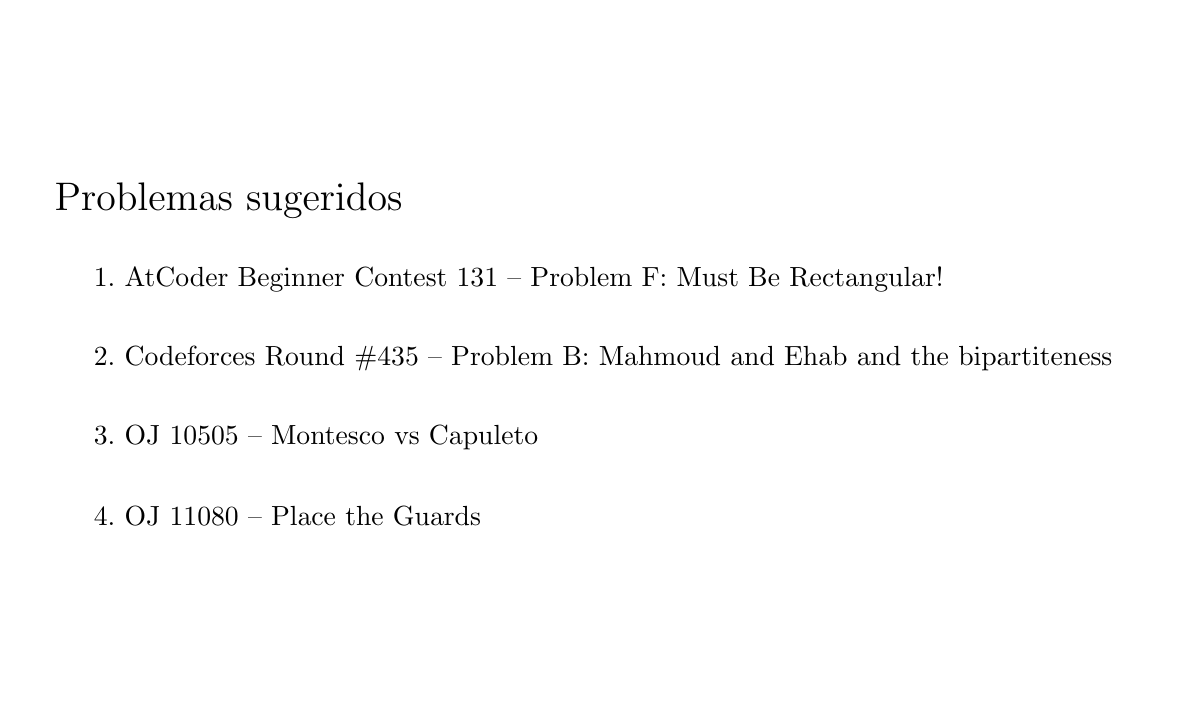
\begin{tikzpicture}
\node[draw,opacity=0] at (0, 0) {x};
\node[draw,opacity=0] at (14, 8) {x};
 \node[anchor=west] at (0, 6) { \Large \bbbold{Problemas sugeridos} };
 \node[anchor=west] at (0.5, 5) { $1.$ \bbtext{AtCoder Beginner Contest 131 -- Problem F: Must Be Rectangular! } };
 \node[anchor=west] at (0.5, 4) { $2.$ \bbtext{Codeforces Round \#435 -- Problem B: Mahmoud and Ehab and the bipartiteness} };
 \node[anchor=west] at (0.5, 3) { $3.$ \bbtext{OJ 10505 -- Montesco vs Capuleto} };
 \node[anchor=west] at (0.5, 2) { $4.$ \bbtext{OJ 11080 -- Place the Guards} };
\end{tikzpicture}
\end{frame}

\begin{frame}[plain,t]

\begin{tikzpicture}
\node[draw,opacity=0] at (0, 0) {x};
\node[draw,opacity=0] at (14, 8) {x};
 \node[anchor=west] at (0, 6) { \Large \bbbold{Referências} };
 \node[anchor=west] at (1, 5) { $1.$ \bbbold{HALIM}, \bbtext{Felix}; \bbbold{HALIM}, \bbtext{Steve}. \bbenglish{Competitive Programming 3,} \bbtext{2010.} };
 \node[anchor=west] at (1, 4) { $2.$ \bbbold{LAAKSONEN}, \bbtext{Antti}. \bbenglish{Competitive Programmer's Handbook,} \bbtext{2018.} };
 \node[anchor=west] at (1, 3) { $3.$ \bbbold{SKIENA}, \bbtext{Steven}; \bbbold{REVILLA}, \bbtext{Miguel}. \bbenglish{Programming Challenges,} \bbtext{2003.} };
\end{tikzpicture}
\end{frame}

\end{document}
